\documentclass[10pt,a4paper]{article} % font size + paper
\usepackage[margin=2cm]{geometry} % setting up geometry
\usepackage{graphicx}
\usepackage{helvet} % using helvetica-like font
\usepackage[colorlinks=false]{hyperref} % for links
% for the content
\usepackage{array, xcolor}
\definecolor{lightgray}{gray}{0.8}
\newcolumntype{L}{>{\raggedleft}p{0.14\textwidth}}
\newcolumntype{R}{p{0.8\textwidth}}
\newcommand\VRule{\color{lightgray}\vrule width 0.5pt}
\usepackage{natbib}
\usepackage{bibentry}

%%% Example how to add content %%%

%\section*{Heading}
% \begin{tabular}{L!{\VRule}R}
%  2012&Some text\\[5pt]
%  2011&Some other text\\
% \end{tabular}

% for try out
\usepackage{lipsum}

% headers
\usepackage{fancyhdr}
\pagestyle{fancy}
\rfoot{Barcelona, Spain}
\lfoot{\today}
\renewcommand{\headrulewidth}{0pt}
\renewcommand{\footrulewidth}{0pt}

% name
\title{\bfseries\Huge David Mas-Ponte}
% Job
\author{Bioinformatician}
% today's date
\date{}

% fonts
 \renewcommand{\familydefault}{\sfdefault}

%img path
\graphicspath{{img/}}

\begin{document}

% Header
\begin{minipage}[c]{0.65\textwidth}
% make title puts the name and mail in the left
\maketitle
\end{minipage}
\begin{minipage}[c]{0.3\textwidth}
%profile picture
  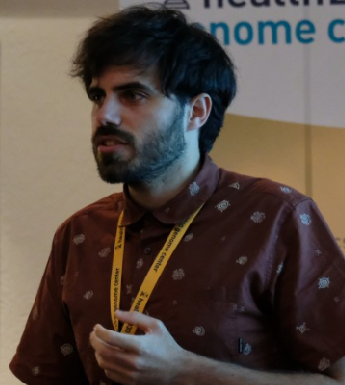
\includegraphics[width=.55\textwidth]{profile}
\end{minipage}


% Subheader
\begin{minipage}[c]{0.65\textwidth}
  \begin{center}
    \href{mailto:david.mas.p@gmail.com}{david.mas.p@gmail.com}\\
    +34 662 612 983\\
    Barcelona, Spain
  \end{center}
\end{minipage}
\begin{minipage}[c]{0.3\textwidth}
\href{https://github.com/davidmasp}{github://davidmasp}

\includegraphics[height=12pt]{gh}\\
\href{https://www.linkedin.com/in/davidmasponte/}{linkedin://davidmasponte}

\includegraphics[height=12pt]{in}\\
\href{https://davidmasp.github.io}{davidmasp.github.io}
\end{minipage}


\vspace{0.75cm}
\rule{.95\textwidth}{0.6pt}

%%%% EDUCATION %%%%

\section*{Education}
\begin{tabular}{L!{\VRule}R}
  2015--2017&{\bf M.Sc. in Bioinformatics for Health Science}\\
   & Universitat Pompeu Fabra, Barcelona, Spain.\\
   & {\em \color{black!50} Specialization in Genomics - GPA: 9 / 10 }\\[15pt]
  2014&Exchange Student \\
   &  McGill University, Montreal, Canada.\\
   & {\em \color{black!50} Academic international exchange}\\[15pt]
  2011--2015&B.Sc. in Biotechnology\\
   & Universitat Autonoma de Barcelona, Spain.\\
   & { \em \color{black!50} GPA: 8.5 / 10}
\end{tabular}

%%%% Research %%%%
\section*{Research Experience}
\begin{tabular}{L!{\VRule}R}
Jul 2016-today&{\bf Centre for Genomic Regulation (CRG) } - {\em \color{black!70} Master Science Research Thesis  }\\
 & My Master Thesis is focused in the link between lncRNAs\' subcellular localization and their function. I have also developed a web-based DB using R and SQL to make subcellular data available to the scientific community. {\bf Roderic Guigo’ Lab, tutored by Rory Johnson}.\\[15pt]
2015-2016 & {\bf Institute of Evolutionary Biology (IBE) } - {\em \color{black!70} Part time Research Internship}\\
 & I studied the evolutionary processes surrounding the RHD gene in Western Mediterranean populations in order to unravel demographic ({\em drift}) or adaptive ({\em selection}) processes round this locus. {\bf David Comas\' Lab}\\[15pt]
06-08 2014 & {\bf Molecular Biology Institute of Barcelona (IBMB) }- {\em \color{black!70} Research Internship}\\
 &  I took part in the study of the CIC (CapICua) protein in Drosophila development. I gained research skills in fruit  y genetics, in in situ hybridization and in recombinant DNA techniques for CRISPR/Cas9 set up. {\bf Gerardo Jimenez’s Lab}
\end{tabular}


%%%% Programing %%%%
\section*{Code}
\begin{tabular}{L!{\VRule}R}
  Good & python, SQL, R \& git \\
  Fair & Perl, Shell \& \LaTeX \\
  Learning & Ruby \& JavaScript (D3)
\end{tabular}


%%%% pubs %%%%

\bibliographystyle{unsrtnat}
\nobibliography{dmas201701}

\section*{Publications \& Conferences}
\begin{tabular}{L!{\VRule}R}
2017&\bibentry{dmas201701} - {\em \color{black!70} Submitted}\\[5pt]
2016&\bibentry{flores-bello2016} - {\em \color{black!70} Peer-reviewed Conference - Poster}\\
\end{tabular}



%%%% lang %%%%
\section*{Languages}
\begin{tabular}{L!{\VRule}R}
Catalan & Mother tongue\\
Spanish & Bilingual Proficiency\\
{\bf English}&{\bf Fluent (FCE 2011)}
\end{tabular}


%%%% SA %%%%
\section*{Scholarships \& Awards}
  \begin{tabular}{L!{\VRule}R}
    2015-2016 & MECD - COLAB - {\em \color{black!70} Scholarship }\\
     & { \color{black!70} I was awarded with the Beca de Colaboración (Collaboration Scholarship) in Department of Experimental and Health Sciences UPF by Ministerio de Educación, Cultura y Deporte to collaborate in David Comas’ Lab.}\\[15pt]
    Sep-Oct 2015 & JAE INTRO - CSIC - {\em \color{black!70} Scholarship }\\
     & { \color{black!70} I was awarded with a JAE INTRO scholarship in Institute of Evolutionary Biology by Consejo Superior de Investigaciones Cientificas (CSIC) to collaborate in David Comas’ Lab.}\\[15pt]
    2014-2015 & UAB + AGAUR Exchange - {\em \color{black!70} Scholarship}\\
     & { \color{black!70} I was awarded with a scholarship from my university and from the Catalan government for my Exchange Academic Experience in CANADA.}\\[15pt]
    Jul-Ago 2014 & Passa l’estiu al parc-PCB - {\em \color{black!70} Scholarship}\\
     & { \color{black!70} I was awarded with the scholarship Passa l’estiu al parc by Barcelona Science Park (PCB) to collaborate in Gerardo Jimenez’s Lab.}\\[15pt]
    2013 & VI Premi de Recerca en Ciencies de la Salut-PRBB - {\em \color{black!70} Award}\\
     & { \color{black!70} I received the VI Premi de Recerca en Ciencies de la Salut (Research Award in Health Science) by Research Park of Biomedicine in Barcelona (PRBB) for my research project of my baccalaureate "{\em Polymorphism in the CCR5 gene}".}
  \end{tabular}

\end{document}
